\chapter{Design}
%3693 words before this section
%4104 by next day
This chapter covers the design process of the study, including the 

\begin{figure}[!hb]
\centering
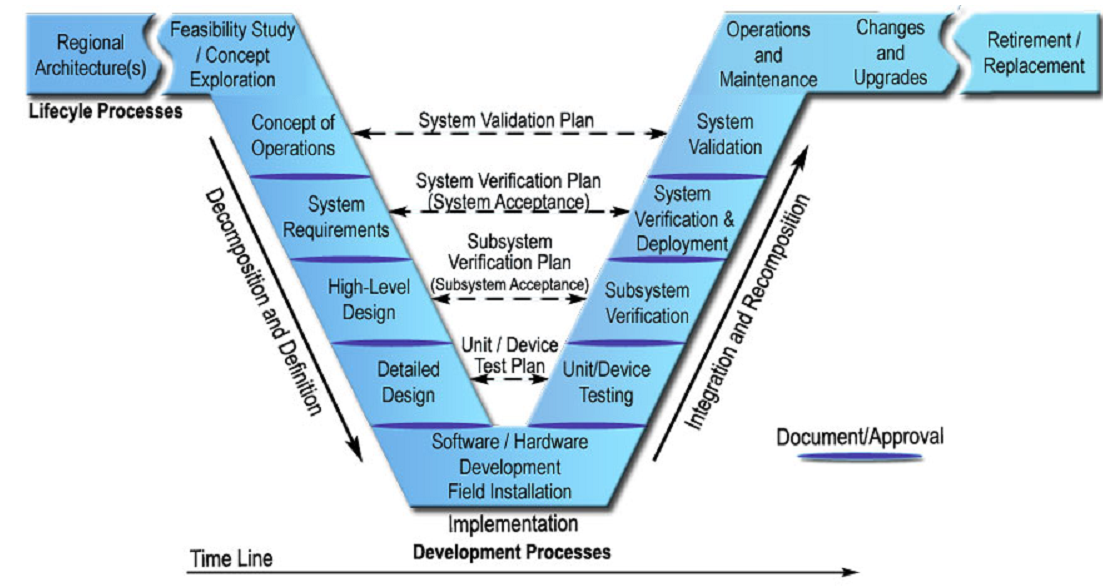
\includegraphics[scale=0.5]{figures/vee_diagram} % will design own diagram
\caption{Vee Diagram}
\label{fig:vee_diagram}
\centering
\end{figure}



\section{Design Context}
This study is within the scope of an undergraduate level approach to both radar and machine learning, with an emphasis on machine learning; the techniques applied herewith are not limited to radar imagery, but attempts should be made to tailor the design to radar applications. With development this study should be adaptable to commercial use, and be helpful to people in the radar department who need assistance with radar target classification. Thus the study should develop an easily extensible framework for radar image classification, or at least guidelines to allow others to integrate with the work covered herein.


\section{Feasibility Study / Concept Exploration}

\section{Decomposition and Definition}
This section is devoted to describing the study in terms of its requirements, operation, and implementation. An accompaniment explaining the verification and validity of each subsection will be in the next section.
\subsection{Concept of Operations}
Radar target classification is an inexact science; interpreting a radar image and comparing it to a known case is not as straightforward in all cases as one might expect. Weather conditions, environmental clutter, and image resolution all obscure the target to varying degrees, making intuitive classification ineffective. Computer-based classification through analysis of multiple targets and the application of deep learning techniques should in theory allow distorted images to be classified after the computer is trained to recognise features pertaining to each class. Na{\"i}ve methods of classification lack predictive power - the ability to 'guess' effectively if the target is obscured or unrecognised. Deep learning methods are the solution that this study proposes.

\subsection{System Requirements}
% insert user requirements from the PDF I've written up elsewhere
% emphasis on accuracy, testing time, and training time
\subsection{High-Level Design}
For this study, these areas of design need to be focused on:
\begin{itemize}
	\item Image Processing/Preparation
	\item Further Dimensionality Reduction
	\item Na{\"i}ve Classification (Nearest Neighbour as a benchmark)
	\item Deep Learning Classification (Multilayer Perceptron)
\end{itemize}



\subsection{Detailed Design}
\subsubsection{Image Processing/Preparation}\label{sec:cropping}
The MSTAR dataset is a compilation of image chips, all of which contain a header, as well as magnitude and phase data. The images are between 54x54 and 192x193 pixels in size, which suggests that some form of image processing should be performed to make sure that all images are the same size. The targets in each image chip are centred, suggesting that cropping each image to a size where the target (and its shadow - useful in classification) are left whole, and as much of the surrounding clutter as possible is removed.

An alternate approach is to retain the data inherent in the environmental clutter and pad the smaller images with zeros, keeping all images in the set at the size of the largest image in the set. While this preserves all of the image chip data, processing larger images leads to infeasibly long training and classification times.

To accurately preserve the data while making the image as small as possible, the images will be cropped in a rectangular box, containing the target and its shadow. The crop dimensions will be chosen to consider all of the image chips. Further processing of the images may be done, to allow for quicker classification of a larger number of images.

\subsubsection{Dimensionality Reduction}
%TODO: find cropped image size!
Each pixel in an image is taken as an feature, forming a feature vector with a length equal to the total number of pixels in the image. The image cropping mentioned in section \ref{sec:cropping} is very effective at reducing the size of this feature vector. The image size is reduced to ---------- (a total of ----- features). This can be reduced further through the application of dimensionality reduction techniques, such as PCA, LLE, SOM and non-linear methods. 

The first foray into dimensionality reduction will be conducted using PCA techniques \ref{lit:PCA}(cover in the literature review)

\subsubsection{Nearest Neighbour Design}
\begin{figure}
\centering
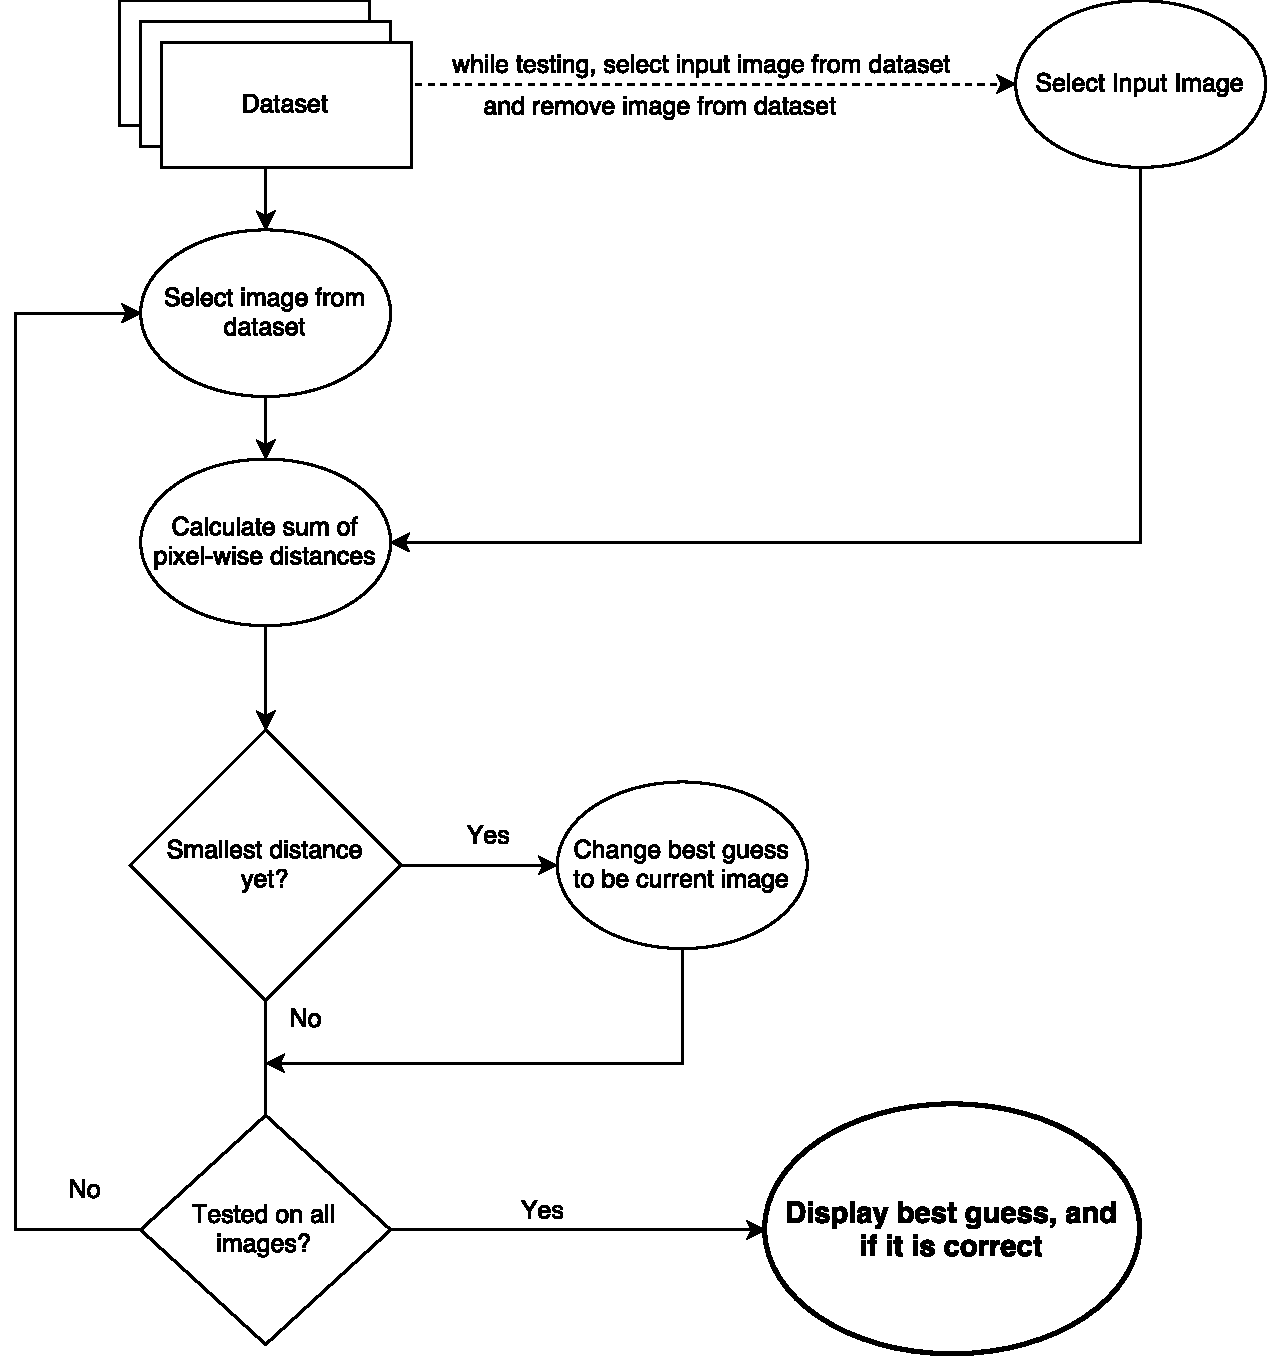
\includegraphics[width=\textwidth]{figures/nearest-neighbour}
\label{fig:nn}
\caption{Nearest Neighbour Classification Flow Diagram}
\centering
\end{figure}


The high-level design is fairly straightforward, and is shown in figure~\ref{fig:nn}. Its principles of operation are covered in section~\ref{lit:nn}. To implement this classifier, the following is needed:

\begin{itemize}
	\item Access to the dataset
	\item A choice of input image
	\item A method to calculate and sum the pixel-wise distances
	\item A variable storing the smallest distance and tentative classification
	\item A method displaying the chosen class and whether or not it is correct
\end{itemize}


\subsubsection{Multilayer Perceptron Design}

Implementation of a multilayer perceptron in software can be divided into discrete sections as follows:
\begin{itemize}
	\item
	
	
	
	
\end{itemize}


\subsection{Software Development and Implementation}




-----
The software present in this study has been made \href{http://github.com/roansong}{available on Github}

\section{Integration and Recomposition}
\subsection{Software Development and Implementation}
\subsubsection{Algorithm Testing}
For each classifier, their effectiveness on the MSTAR dataset must be tested and catalogued, beginning with the Nearest Neighbour implementation. Doing the Nearest Neighbour classification first establishes a benchmark against which further methods can be tested. The na{\"i}ve nature of the Nearest Neighbour classifier means that it is not optimised for any particular dataset. It shows the efficacy of a generic algorithm applied to the MSTAR dataset.

For the effectiveness of any algorithm to be tested, correct and incorrect outputs must be defined. The MSTAR dataset includes target labels in a header section of each file, but since the operations are conducted on files with their header and phase data stripped away it merely adds computational complexity to find the corresponding header for each file and then parse it to extract data about each target. To simplify classification, a variant of a one-hot vector denoting the classes is attached to each target.The vector consists of a series of numbers, equal in length to the number of classes in the dataset. A '1' denotes that the instance is a member of the class corresponding to that entry in the vector, and the rest of the numbers are -1, showing that the instance is not in those classes. A file is created listing all of the filenames to be tested during the run of the algorithm. An example file with ten entries and two classes would look as follows:\\

\begin{center}
\begin{tabular}{c}
HB03333.003.tiff 1 -1 \\
HB03334.003.tiff 1 -1 \\
HB03335.003.tiff 1 -1 \\
HB03337.003.tiff 1 -1 \\
HB03338.003.tiff 1 -1 \\
HB14931.025.tiff -1 1 \\
HB14932.025.tiff -1 1 \\
HB14933.025.tiff -1 1 \\
HB14934.025.tiff -1 1 \\
HB14935.025.tiff -1 1 \\


\end{tabular}
\end{center}

\subsubsection{Testing During Development}
The simplest way to find a classifier's efficacy is to test it on a wide variety of classes and on as many test instances as possible. To provide interim results, during the iterative phase of classifier development, only a subset of the dataset's images are used. This compromises the final accuracy of the classifier (it may perform differently on the full dataset), but bring with it the ability to test and train classifiers more quickly, due to the lower computational overheads. During the development this testing method allows for simple decisions regarding the direction of classifier implementation or optimisation to be made. In process of verifying the classifiers, the full dataset must be used to give an accurate picture of the classifier's performance and real-world implementation. 

\subsection{Subsystem Verification}
The chosen method for verifying a classifier's efficacy once it is considered to be sufficiently optimised is simple; The classifier is tested on the dataset with a number of test instances; if time allows, leave-one-out cross-correlation (LOOCV) covered in section~\ref{lit:loocv} will be used. This entails removing one instance from the dataset, training the classifier on the remaining points, and using the removed instance as a test case. Once this has been done, the instance is replaced, another is taken, and the process is repeated until every instance in the dataset has been tested. The system's performance is based on the number of correct classifications made during the process, and also gives a good estimate of the Separability Index of the data (section~\ref{lit:SI}. 
\subsection{System Verification and Deployment}
\subsection{System Validation}
\subsection{Operations and Maintenance}
\subsection{Changes and Upgrades}
\subsection{Retirement / Replacement}












